\documentclass[twoside]{book}

% Packages required by doxygen
\usepackage{fixltx2e}
\usepackage{calc}
\usepackage{doxygen}
\usepackage[export]{adjustbox} % also loads graphicx
\usepackage{graphicx}
\usepackage[utf8]{inputenc}
\usepackage{makeidx}
\usepackage{multicol}
\usepackage{multirow}
\PassOptionsToPackage{warn}{textcomp}
\usepackage{textcomp}
\usepackage[nointegrals]{wasysym}
\usepackage[table]{xcolor}

% Font selection
\usepackage[T1]{fontenc}
\usepackage[scaled=.90]{helvet}
\usepackage{courier}
\usepackage{amssymb}
\usepackage{sectsty}
\renewcommand{\familydefault}{\sfdefault}
\allsectionsfont{%
  \fontseries{bc}\selectfont%
  \color{darkgray}%
}
\renewcommand{\DoxyLabelFont}{%
  \fontseries{bc}\selectfont%
  \color{darkgray}%
}
\newcommand{\+}{\discretionary{\mbox{\scriptsize$\hookleftarrow$}}{}{}}

% Page & text layout
\usepackage{geometry}
\geometry{%
  a4paper,%
  top=2.5cm,%
  bottom=2.5cm,%
  left=2.5cm,%
  right=2.5cm%
}
\tolerance=750
\hfuzz=15pt
\hbadness=750
\setlength{\emergencystretch}{15pt}
\setlength{\parindent}{0cm}
\setlength{\parskip}{3ex plus 2ex minus 2ex}
\makeatletter
\renewcommand{\paragraph}{%
  \@startsection{paragraph}{4}{0ex}{-1.0ex}{1.0ex}{%
    \normalfont\normalsize\bfseries\SS@parafont%
  }%
}
\renewcommand{\subparagraph}{%
  \@startsection{subparagraph}{5}{0ex}{-1.0ex}{1.0ex}{%
    \normalfont\normalsize\bfseries\SS@subparafont%
  }%
}
\makeatother

% Headers & footers
\usepackage{fancyhdr}
\pagestyle{fancyplain}
\fancyhead[LE]{\fancyplain{}{\bfseries\thepage}}
\fancyhead[CE]{\fancyplain{}{}}
\fancyhead[RE]{\fancyplain{}{\bfseries\leftmark}}
\fancyhead[LO]{\fancyplain{}{\bfseries\rightmark}}
\fancyhead[CO]{\fancyplain{}{}}
\fancyhead[RO]{\fancyplain{}{\bfseries\thepage}}
\fancyfoot[LE]{\fancyplain{}{}}
\fancyfoot[CE]{\fancyplain{}{}}
\fancyfoot[RE]{\fancyplain{}{\bfseries\scriptsize Generated by Doxygen }}
\fancyfoot[LO]{\fancyplain{}{\bfseries\scriptsize Generated by Doxygen }}
\fancyfoot[CO]{\fancyplain{}{}}
\fancyfoot[RO]{\fancyplain{}{}}
\renewcommand{\footrulewidth}{0.4pt}
\renewcommand{\chaptermark}[1]{%
  \markboth{#1}{}%
}
\renewcommand{\sectionmark}[1]{%
  \markright{\thesection\ #1}%
}

% Indices & bibliography
\usepackage{natbib}
\usepackage[titles]{tocloft}
\setcounter{tocdepth}{3}
\setcounter{secnumdepth}{5}
\makeindex

% Hyperlinks (required, but should be loaded last)
\usepackage{ifpdf}
\ifpdf
  \usepackage[pdftex,pagebackref=true]{hyperref}
\else
  \usepackage[ps2pdf,pagebackref=true]{hyperref}
\fi
\hypersetup{%
  colorlinks=true,%
  linkcolor=blue,%
  citecolor=blue,%
  unicode%
}

% Custom commands
\newcommand{\clearemptydoublepage}{%
  \newpage{\pagestyle{empty}\cleardoublepage}%
}

\usepackage{caption}
\captionsetup{labelsep=space,justification=centering,font={bf},singlelinecheck=off,skip=4pt,position=top}

%===== C O N T E N T S =====

\begin{document}

% Titlepage & ToC
\hypersetup{pageanchor=false,
             bookmarksnumbered=true,
             pdfencoding=unicode
            }
\pagenumbering{alph}
\begin{titlepage}
\vspace*{7cm}
\begin{center}%
{\Large My Project }\\
\vspace*{1cm}
{\large Generated by Doxygen 1.8.13}\\
\end{center}
\end{titlepage}
\clearemptydoublepage
\pagenumbering{roman}
\tableofcontents
\clearemptydoublepage
\pagenumbering{arabic}
\hypersetup{pageanchor=true}

%--- Begin generated contents ---
\chapter{Hierarchical Index}
\section{Class Hierarchy}
This inheritance list is sorted roughly, but not completely, alphabetically\+:\begin{DoxyCompactList}
\item \contentsline{section}{Genfun\+:\+:Argument}{\pageref{classGenfun_1_1Argument}}{}
\item \contentsline{section}{background\+\_\+task}{\pageref{classbackground__task}}{}
\item \contentsline{section}{Core}{\pageref{classCore}}{}
\begin{DoxyCompactList}
\item \contentsline{section}{Audit}{\pageref{classAudit}}{}
\item \contentsline{section}{Audit}{\pageref{classAudit}}{}
\item \contentsline{section}{Grad}{\pageref{classGrad}}{}
\item \contentsline{section}{Grad}{\pageref{classGrad}}{}
\item \contentsline{section}{Pass\+Fail}{\pageref{classPassFail}}{}
\item \contentsline{section}{Pass\+Fail}{\pageref{classPassFail}}{}
\end{DoxyCompactList}
\item \contentsline{section}{Initiate\+Vector\+Method$<$ Item\+Type $>$}{\pageref{classInitiateVectorMethod}}{}
\item \contentsline{section}{M\+P\+I\+\_\+\+B\+C\+\_\+\+Generic$<$ T, Q, R $>$}{\pageref{classMPI__BC__Generic}}{}
\item \contentsline{section}{M\+P\+I\+\_\+sorting\+\_\+methods}{\pageref{classMPI__sorting__methods}}{}
\item \contentsline{section}{O\+MP$<$ T $>$}{\pageref{classOMP}}{}
\item \contentsline{section}{Partstruct}{\pageref{structPartstruct}}{}
\item \contentsline{section}{part1\+:\+:Point}{\pageref{classpart1_1_1Point}}{}
\item \contentsline{section}{Prob\+Dist}{\pageref{classProbDist}}{}
\item \contentsline{section}{Progression}{\pageref{classProgression}}{}
\begin{DoxyCompactList}
\item \contentsline{section}{Arith\+Progression}{\pageref{classArithProgression}}{}
\end{DoxyCompactList}
\item \contentsline{section}{Q\+Tstyle\+\_\+\+Test}{\pageref{classQTstyle__Test}}{}
\item \contentsline{section}{Random\+Number\+Generator}{\pageref{classRandomNumberGenerator}}{}
\item \contentsline{section}{Stack$<$ T, C\+O\+NT $>$}{\pageref{classStack}}{}
\item \contentsline{section}{Statistical\+Distribution}{\pageref{classStatisticalDistribution}}{}
\begin{DoxyCompactList}
\item \contentsline{section}{Standard\+Normal\+Distribution}{\pageref{classStandardNormalDistribution}}{}
\end{DoxyCompactList}
\item \contentsline{section}{Str}{\pageref{classStr}}{}
\item \contentsline{section}{Student\+\_\+info}{\pageref{classStudent__info}}{}
\item \contentsline{section}{Template\+Under\+Test$<$ T $>$}{\pageref{classTemplateUnderTest}}{}
\item Test\+Case\begin{DoxyCompactList}
\item \contentsline{section}{M\+P\+I\+\_\+\+BC}{\pageref{classMPI__BC}}{}
\item \contentsline{section}{M\+P\+I\+Input}{\pageref{classMPIInput}}{}
\item \contentsline{section}{Vec$<$ T $>$}{\pageref{classVec}}{}
\item \contentsline{section}{Vec$<$ char $>$}{\pageref{classVec}}{}
\end{DoxyCompactList}
\item Test\+Fixture\begin{DoxyCompactList}
\item \contentsline{section}{Vector\+Method\+Test}{\pageref{classVectorMethodTest}}{}
\end{DoxyCompactList}
\item \contentsline{section}{Trap}{\pageref{classTrap}}{}
\item \contentsline{section}{tutorial\+:\+:Vec$<$ T $>$}{\pageref{classtutorial_1_1Vec}}{}
\end{DoxyCompactList}

\chapter{Class Index}
\section{Class List}
Here are the classes, structs, unions and interfaces with brief descriptions\+:\begin{DoxyCompactList}
\item\contentsline{section}{\hyperlink{structbinary}{binary$<$ N $>$} }{\pageref{structbinary}}{}
\item\contentsline{section}{\hyperlink{structbinary_3_010_01_4}{binary$<$ 0 $>$} }{\pageref{structbinary_3_010_01_4}}{}
\item\contentsline{section}{\hyperlink{classDistance}{Distance} }{\pageref{classDistance}}{}
\item\contentsline{section}{\hyperlink{structfunc}{func} }{\pageref{structfunc}}{}
\item\contentsline{section}{\hyperlink{structis__incrementable}{is\+\_\+incrementable$<$ typename, typename $>$} }{\pageref{structis__incrementable}}{}
\item\contentsline{section}{\hyperlink{structis__incrementable_3_01T_00_01std_1_1void__t_3_01decltype_07_09_09std_1_1declval_3_01T_01_6_01_4_07_08_08_4_01_4}{is\+\_\+incrementable$<$ T, std\+::void\+\_\+t$<$ decltype(++std\+::declval$<$ T \& $>$())$>$ $>$} }{\pageref{structis__incrementable_3_01T_00_01std_1_1void__t_3_01decltype_07_09_09std_1_1declval_3_01T_01_6_01_4_07_08_08_4_01_4}}{}
\item\contentsline{section}{\hyperlink{structless}{less$<$ T $>$} }{\pageref{structless}}{}
\item\contentsline{section}{\hyperlink{classthread__guard}{thread\+\_\+guard} }{\pageref{classthread__guard}}{}
\end{DoxyCompactList}

\chapter{Class Documentation}
\hypertarget{structbinary}{}\section{binary$<$ N $>$ Struct Template Reference}
\label{structbinary}\index{binary$<$ N $>$@{binary$<$ N $>$}}
\subsection*{Static Public Attributes}
\begin{DoxyCompactItemize}
\item 
static unsigned const {\bfseries value}
\end{DoxyCompactItemize}


\subsection{Member Data Documentation}
\mbox{\Hypertarget{structbinary_a945f31f5adc56b48f3ded51940ec75b3}\label{structbinary_a945f31f5adc56b48f3ded51940ec75b3}} 
\index{binary@{binary}!value@{value}}
\index{value@{value}!binary@{binary}}
\subsubsection{\texorpdfstring{value}{value}}
{\footnotesize\ttfamily template$<$unsigned long N$>$ \\
unsigned const \hyperlink{structbinary}{binary}$<$ N $>$\+::value\hspace{0.3cm}{\ttfamily [static]}}

{\bfseries Initial value\+:}
\begin{DoxyCode}
= \hyperlink{structbinary}{binary}<N/10>::value << 1 
               | N%10
\end{DoxyCode}


The documentation for this struct was generated from the following file\+:\begin{DoxyCompactItemize}
\item 
/home/oohnohnoh1/\+Desktop/\+G\+I\+T/\+Research/\+Pthreads\+\_\+work/Metaprogramming1.\+cxx\end{DoxyCompactItemize}

\hypertarget{structbinary_3_010_01_4}{}\section{binary$<$ 0 $>$ Struct Template Reference}
\label{structbinary_3_010_01_4}\index{binary$<$ 0 $>$@{binary$<$ 0 $>$}}
\subsection*{Static Public Attributes}
\begin{DoxyCompactItemize}
\item 
\mbox{\Hypertarget{structbinary_3_010_01_4_aff4cd37ff042fbf643ce6816df9f6f16}\label{structbinary_3_010_01_4_aff4cd37ff042fbf643ce6816df9f6f16}} 
static unsigned const {\bfseries value} = 0
\end{DoxyCompactItemize}


The documentation for this struct was generated from the following file\+:\begin{DoxyCompactItemize}
\item 
/home/oohnohnoh1/\+Desktop/\+G\+I\+T/\+Research/\+Pthreads\+\_\+work/Metaprogramming1.\+cxx\end{DoxyCompactItemize}

\hypertarget{classDistance}{}\section{Distance Class Reference}
\label{classDistance}\index{Distance@{Distance}}
\subsection*{Public Member Functions}
\begin{DoxyCompactItemize}
\item 
\mbox{\Hypertarget{classDistance_a486dd7fdd83bca097941986f42ac3107}\label{classDistance_a486dd7fdd83bca097941986f42ac3107}} 
{\bfseries Distance} (int f, int i)
\item 
\mbox{\Hypertarget{classDistance_ad89badc4cbfaa5c27b0b2f8205ac2da8}\label{classDistance_ad89badc4cbfaa5c27b0b2f8205ac2da8}} 
\hyperlink{classDistance}{Distance} {\bfseries operator()} (int a, int b, int c)
\item 
\mbox{\Hypertarget{classDistance_a396afa4e4499b1e7f11c1c56d332adce}\label{classDistance_a396afa4e4499b1e7f11c1c56d332adce}} 
void {\bfseries display\+Distance} ()
\end{DoxyCompactItemize}


The documentation for this class was generated from the following file\+:\begin{DoxyCompactItemize}
\item 
/home/oohnohnoh1/\+Desktop/\+G\+I\+T/\+Research/\+Pthreads\+\_\+work/Managing\+Threads1.\+cxx\end{DoxyCompactItemize}

\hypertarget{structfunc}{}\section{func Struct Reference}
\label{structfunc}\index{func@{func}}
\subsection*{Public Member Functions}
\begin{DoxyCompactItemize}
\item 
\mbox{\Hypertarget{structfunc_a6801d59dec3f95f3f7e2d9505212f144}\label{structfunc_a6801d59dec3f95f3f7e2d9505212f144}} 
{\bfseries func} (int \&i\+\_\+)
\item 
\mbox{\Hypertarget{structfunc_ae6878437e9e8405fe4f96dd798ef835d}\label{structfunc_ae6878437e9e8405fe4f96dd798ef835d}} 
void {\bfseries operator()} ()
\item 
\mbox{\Hypertarget{structfunc_a6801d59dec3f95f3f7e2d9505212f144}\label{structfunc_a6801d59dec3f95f3f7e2d9505212f144}} 
{\bfseries func} (int \&i\+\_\+)
\item 
\mbox{\Hypertarget{structfunc_ae6878437e9e8405fe4f96dd798ef835d}\label{structfunc_ae6878437e9e8405fe4f96dd798ef835d}} 
void {\bfseries operator()} ()
\end{DoxyCompactItemize}
\subsection*{Public Attributes}
\begin{DoxyCompactItemize}
\item 
\mbox{\Hypertarget{structfunc_af3b5e33f274c8e00a4e44cb5893e0f47}\label{structfunc_af3b5e33f274c8e00a4e44cb5893e0f47}} 
int \& {\bfseries i}
\end{DoxyCompactItemize}


The documentation for this struct was generated from the following files\+:\begin{DoxyCompactItemize}
\item 
/home/oohnohnoh1/\+Desktop/\+G\+I\+T/\+Research/\+Pthreads\+\_\+work/Managing\+Threads1.\+cxx\item 
/home/oohnohnoh1/\+Desktop/\+G\+I\+T/\+Research/\+Pthreads\+\_\+work/S\+Y\+N\+\_\+thread1.\+cxx\end{DoxyCompactItemize}

\hypertarget{structis__incrementable}{}\section{is\+\_\+incrementable$<$ typename, typename $>$ Struct Template Reference}
\label{structis__incrementable}\index{is\+\_\+incrementable$<$ typename, typename $>$@{is\+\_\+incrementable$<$ typename, typename $>$}}


Inheritance diagram for is\+\_\+incrementable$<$ typename, typename $>$\+:
\nopagebreak
\begin{figure}[H]
\begin{center}
\leavevmode
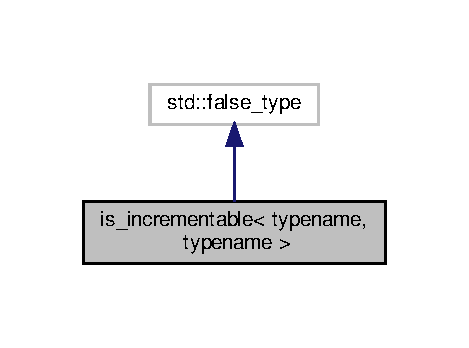
\includegraphics[width=225pt]{structis__incrementable__inherit__graph}
\end{center}
\end{figure}


Collaboration diagram for is\+\_\+incrementable$<$ typename, typename $>$\+:
\nopagebreak
\begin{figure}[H]
\begin{center}
\leavevmode
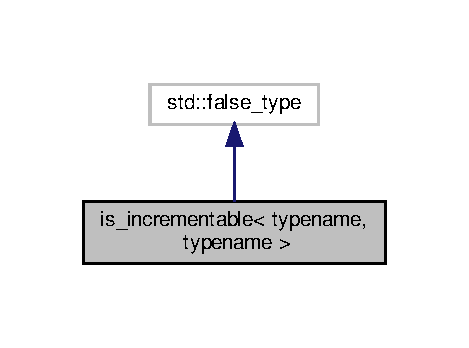
\includegraphics[width=225pt]{structis__incrementable__coll__graph}
\end{center}
\end{figure}


The documentation for this struct was generated from the following file\+:\begin{DoxyCompactItemize}
\item 
/home/oohnohnoh1/\+Desktop/\+G\+I\+T/\+Research/\+Pthreads\+\_\+work/Metaprogramming1.\+cxx\end{DoxyCompactItemize}

\hypertarget{structis__incrementable_3_01T_00_01std_1_1void__t_3_01decltype_07_09_09std_1_1declval_3_01T_01_6_01_4_07_08_08_4_01_4}{}\section{is\+\_\+incrementable$<$ T, std\+:\+:void\+\_\+t$<$ decltype(++std\+:\+:declval$<$ T \& $>$())$>$ $>$ Struct Template Reference}
\label{structis__incrementable_3_01T_00_01std_1_1void__t_3_01decltype_07_09_09std_1_1declval_3_01T_01_6_01_4_07_08_08_4_01_4}\index{is\+\_\+incrementable$<$ T, std\+::void\+\_\+t$<$ decltype(++std\+::declval$<$ T \& $>$())$>$ $>$@{is\+\_\+incrementable$<$ T, std\+::void\+\_\+t$<$ decltype(++std\+::declval$<$ T \& $>$())$>$ $>$}}


Inheritance diagram for is\+\_\+incrementable$<$ T, std\+:\+:void\+\_\+t$<$ decltype(++std\+:\+:declval$<$ T \& $>$())$>$ $>$\+:
\nopagebreak
\begin{figure}[H]
\begin{center}
\leavevmode
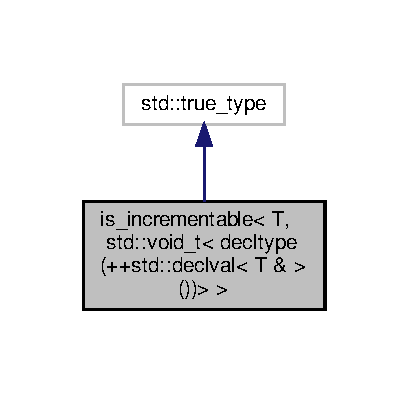
\includegraphics[width=196pt]{structis__incrementable_3_01T_00_01std_1_1void__t_3_01decltype_07_09_09std_1_1declval_3_01T_01_626b84646f93e9036207fd1a3d325191b}
\end{center}
\end{figure}


Collaboration diagram for is\+\_\+incrementable$<$ T, std\+:\+:void\+\_\+t$<$ decltype(++std\+:\+:declval$<$ T \& $>$())$>$ $>$\+:
\nopagebreak
\begin{figure}[H]
\begin{center}
\leavevmode
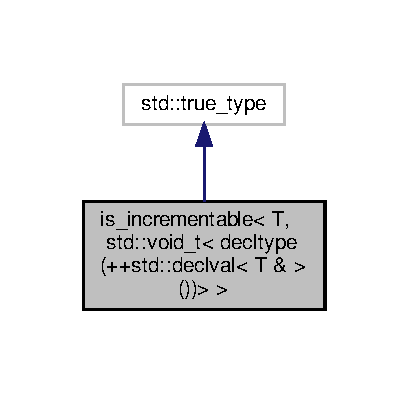
\includegraphics[width=196pt]{structis__incrementable_3_01T_00_01std_1_1void__t_3_01decltype_07_09_09std_1_1declval_3_01T_01_6d213328f6fc3f5a28b2168eb22b51537}
\end{center}
\end{figure}


The documentation for this struct was generated from the following file\+:\begin{DoxyCompactItemize}
\item 
/home/oohnohnoh1/\+Desktop/\+G\+I\+T/\+Research/\+Pthreads\+\_\+work/Metaprogramming1.\+cxx\end{DoxyCompactItemize}

\hypertarget{structless}{}\section{less$<$ T $>$ Struct Template Reference}
\label{structless}\index{less$<$ T $>$@{less$<$ T $>$}}
\subsection*{Public Member Functions}
\begin{DoxyCompactItemize}
\item 
\mbox{\Hypertarget{structless_a087ca6938bbfd0310df3dd3d3e2ff30e}\label{structless_a087ca6938bbfd0310df3dd3d3e2ff30e}} 
bool {\bfseries operator()} (T a, T b) const
\item 
\mbox{\Hypertarget{structless_a087ca6938bbfd0310df3dd3d3e2ff30e}\label{structless_a087ca6938bbfd0310df3dd3d3e2ff30e}} 
bool {\bfseries operator()} (T a, T b) const
\end{DoxyCompactItemize}


The documentation for this struct was generated from the following file\+:\begin{DoxyCompactItemize}
\item 
/home/oohnohnoh1/\+Desktop/\+G\+I\+T/\+Research/\+Pthreads\+\_\+work/Metaprogramming2.\+cxx\end{DoxyCompactItemize}

\hypertarget{classthread__guard}{}\section{thread\+\_\+guard Class Reference}
\label{classthread__guard}\index{thread\+\_\+guard@{thread\+\_\+guard}}
\subsection*{Public Member Functions}
\begin{DoxyCompactItemize}
\item 
\mbox{\Hypertarget{classthread__guard_a4429daa8a5ac0284b12d02170f253823}\label{classthread__guard_a4429daa8a5ac0284b12d02170f253823}} 
{\bfseries thread\+\_\+guard} (std\+::thread \&t\+\_\+)
\end{DoxyCompactItemize}


The documentation for this class was generated from the following file\+:\begin{DoxyCompactItemize}
\item 
/home/oohnohnoh1/\+Desktop/\+G\+I\+T/\+Research/\+Pthreads\+\_\+work/Managing\+Threads1.\+cxx\end{DoxyCompactItemize}

%--- End generated contents ---

% Index
\backmatter
\newpage
\phantomsection
\clearemptydoublepage
\addcontentsline{toc}{chapter}{Index}
\printindex

\end{document}
